\documentclass{article}
\usepackage{tikz}
\usepackage{float}
\usetikzlibrary{positioning, arrows.meta}

\begin{document}
	
In Figure~\ref{fig:pentabox}.
	
\begin{figure}[htpb]
	\centering
	\hspace{-1.8cm}
	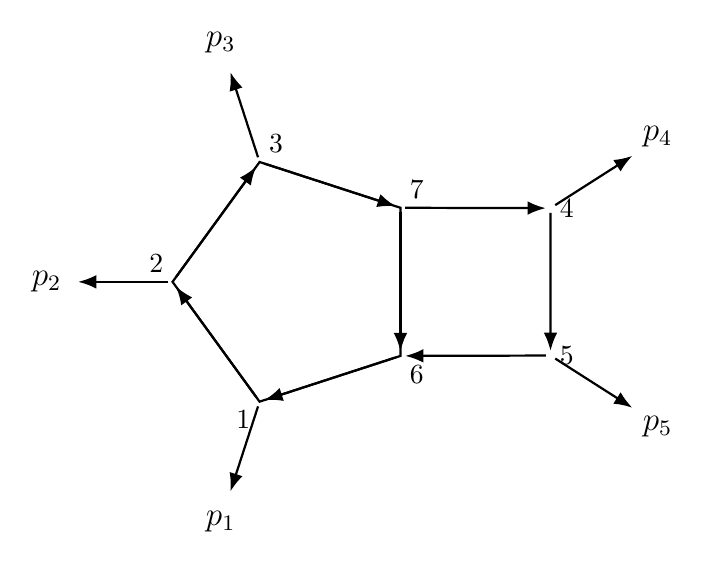
\begin{tikzpicture}[scale=0.8, every node/.style={  inner sep=1.5pt, fill=white}]
		% Define vertices with labels nicely
		\node[label=above right:7] (v7) at (36:2) {};
		\node[label=above right:3] (v3) at (108:2) {};
		\node[label=above left:2] (v2) at (180:2) {};
		\node[label=below left:1] (v1) at (252:2) {};
		\node[label=below right:6] (v6) at (324:2) {};
		\node[label=right:4] (v4) at (4,1.17) {}; % intermediate node
		\node[label=right:5] (v5) at (4,-1.17) {}; % intermediate node

		% Draw pentagon without arrows
		\draw[thick] (v1.center) -- (v2.center) -- (v3.center) -- (v7.center) -- (v6.center) -- cycle;
		
		% Draw external legs
		\draw[thick, -Latex] (v3) -- (108:3.5);  
		\draw[thick, -Latex] (v2) -- (-3.5,0);   
		\draw[thick, -Latex] (v1) -- (252:3.5);  
		\draw[thick, -Latex] (v4) -- (5.3,2);    
		\draw[thick, -Latex] (v5) -- (5.3,-2);   

		% Draw internal directed edges according to e
		\draw[thick, -Latex] (v6) -- (v1);
		\draw[thick, -Latex] (v1) -- (v2);
		\draw[thick, -Latex] (v2) -- (v3);
		\draw[thick, -Latex] (v3) -- (v7);
		\draw[thick, -Latex] (v7) -- (v4);
		\draw[thick, -Latex] (v4) -- (v5);
		\draw[thick, -Latex] (v5) -- (v6);
		\draw[thick, -Latex] (v7) -- (v6);
		
		% External labels
		\node[font=\large\bfseries] at (252:4) {$p_1$};
		\node[font=\large\bfseries] at (-4,0) {$p_2$};
		\node[font=\large\bfseries] at (108:4) {$p_3$};
		\node[font=\large\bfseries] at (5.7,2.3) {$p_4$};
		\node[font=\large\bfseries] at (5.7,-2.3) {$p_5$};
	\end{tikzpicture}
	\caption{A two-loop five-point pentabox diagram with directed edges according to \(e\).}
	\label{fig:pentabox}
\end{figure}
	
\end{document}
